% TODO checklist:
% - [x] Inspected: README.md (typical E2E flows section)
% - [x] Inspected: Q&A.md (Q5: lifecycle of agent run, Q6: lifecycle of background job)
% - [x] Inspected: tests/e2e/test_end_to_end_health.py
% - [x] Inspected: tests/integration/TEST_RESULTS.md
% - [x] Inspected: ui_agent/ (Next.js chat UI flow)
% - [x] Inspected: ui_control_panel/ (Streamlit control panel)

\section{End-to-End Workflows}
\label{sec:e2e-workflows}

This section evaluates the platform's capability to execute complete user workflows from initial request to final response. End-to-end workflows validate the integration of all platform components: authentication, API layer, orchestration, tool invocation, data persistence, and response delivery.

\subsection{Chat / Agent Run Workflow}

The primary user workflow involves submitting a natural language prompt through the chat interface and receiving an agent-generated response. This flow exercises the full agent orchestration pipeline.

\subsubsection{Workflow Steps}

\begin{enumerate}
    \item \textbf{Authentication}: User authenticates via OIDC provider (Auth0) and obtains JWT access token.
    
    \item \textbf{UI Interaction}: User enters prompt in Next.js chat interface and selects target model.
    
    \item \textbf{API Request}: Frontend issues \texttt{POST /v1/agent-runs} with prompt, model selection, and bearer token.
    
    \item \textbf{Security Middleware}: Request passes through JWT validation, tenant extraction, and rate limiting.
    
    \item \textbf{Intent Classification}: Orchestrator classifies prompt intent (CHAT, GRAPH, ADMIN, SECURITY).
    
    \item \textbf{Orchestration}: Multi-step execution with TODO planning, LLM calls, and tool invocations.
    
    \item \textbf{Persistence}: Run state, steps, and metrics are persisted to PostgreSQL.
    
    \item \textbf{Response}: Final output returned to UI with execution trace.
\end{enumerate}

\subsubsection{Validation Criteria}

The agent run workflow is validated against the following criteria:

\begin{table}[ht]
\centering
\caption{Agent run workflow validation criteria.}
\label{tab:agent-run-criteria}
\small
\begin{tabular}{lll}
\hline
\textbf{Criterion} & \textbf{Expected Behavior} & \textbf{Test Method} \\
\hline
Authentication & 401 without token; 200 with valid token & API tests \\
Run creation & Returns \texttt{run\_id} and \texttt{status: pending} & Integration tests \\
Status transitions & \texttt{pending} $\rightarrow$ \texttt{running} $\rightarrow$ \texttt{succeeded/failed} & State machine tests \\
Step recording & All steps persisted with input/output & Database inspection \\
Token counting & Accurate prompt/completion token counts & LLM adapter tests \\
Latency tracking & \texttt{latency\_ms} recorded per step & Metrics validation \\
\hline
\end{tabular}
\end{table}

\subsubsection{Test Results}

End-to-end agent run tests demonstrate:

\begin{itemize}
    \item \textbf{Happy Path}: Chat prompts successfully processed with correct final answers.
    \item \textbf{Error Handling}: Invalid prompts return appropriate RFC 7807 Problem Details.
    \item \textbf{Timeout Behavior}: Long-running prompts respect configured timeouts.
    \item \textbf{Cancellation}: In-progress runs can be cancelled with proper state cleanup.
\end{itemize}

\subsection{Graph Q\&A Workflow}

The graph Q\&A workflow enables natural language queries against the Memgraph knowledge graph through the NL-to-Cypher pipeline.

\subsubsection{Workflow Steps}

\begin{enumerate}
    \item \textbf{Intent Classification}: System identifies GRAPH intent from user prompt.
    
    \item \textbf{Catalog Matching}: Prompt matched against NL prompt catalog for hints.
    
    \item \textbf{Cypher Generation}: LLM generates Cypher query with schema context.
    
    \item \textbf{Safety Validation}: Generated Cypher validated for:
    \begin{itemize}
        \item Read-only enforcement (no WRITE, DELETE, MERGE)
        \item Tenant boundary isolation (\texttt{tenant\_id} filter)
        \item Query depth limits
        \item Timeout guards
    \end{itemize}
    
    \item \textbf{Query Execution}: Validated Cypher executed against Memgraph.
    
    \item \textbf{Result Summarization}: LLM generates natural language summary of results.
\end{enumerate}

\subsubsection{Test Mode for Deterministic Evaluation}

The NL-to-Cypher pipeline supports a test mode for reproducible evaluation:

\begin{lstlisting}[language=Python,caption={NL-to-Cypher test mode configuration.}]
{
    "normalized_prompt": "show all users",
    "expected_cypher": "MATCH (u:User) RETURN u LIMIT 100",
    "expected_intent": "GRAPH",
    "test_context": {
        "tenant_id": "test-tenant"
    }
}
\end{lstlisting}

This enables:
\begin{itemize}
    \item Independence from LLM output variability
    \item Deterministic query validation
    \item Regression testing of Cypher generation
\end{itemize}

\subsubsection{Validation Results}

\begin{table}[ht]
\centering
\caption{Graph Q\&A workflow validation results.}
\label{tab:graph-qa-results}
\small
\begin{tabular}{llc}
\hline
\textbf{Test Case} & \textbf{Description} & \textbf{Status} \\
\hline
Schema queries & ``Show me the graph schema'' & \textcolor{green}{\checkmark} Pass \\
Node listing & ``List all users'' & \textcolor{green}{\checkmark} Pass \\
Relationship traversal & ``Find files created by user X'' & \textcolor{green}{\checkmark} Pass \\
Aggregation & ``Count tasks per institution'' & \textcolor{green}{\checkmark} Pass \\
Write rejection & ``Delete all nodes'' & \textcolor{green}{\checkmark} Pass (blocked) \\
Tenant isolation & Cross-tenant query attempt & \textcolor{green}{\checkmark} Pass (isolated) \\
\hline
\end{tabular}
\end{table}

\subsection{Long-Running Job Workflow}

The job system handles operations that exceed typical request timeouts, with persistent state and progress streaming.

\subsubsection{Workflow Steps}

\begin{enumerate}
    \item \textbf{Job Creation}: Client issues \texttt{POST /v1/jobs} with job type and payload.
    
    \item \textbf{Queue Submission}: Job document created in PostgreSQL; job ID pushed to Redis queue.
    
    \item \textbf{Worker Assignment}: Background worker dequeues job via \texttt{BRPOP}.
    
    \item \textbf{Execution}: Worker processes job with periodic heartbeats.
    
    \item \textbf{Progress Updates}: SSE events streamed via \texttt{GET /v1/jobs/\{id\}/events}.
    
    \item \textbf{Completion}: Final status (\texttt{finished}/\texttt{failed}) persisted; result available via \texttt{GET /v1/jobs/\{id\}}.
\end{enumerate}

\subsubsection{State Machine Validation}

The job state machine enforces valid transitions as shown in Figure~\ref{fig:job-state-machine}.

\begin{figure}[ht]
\centering
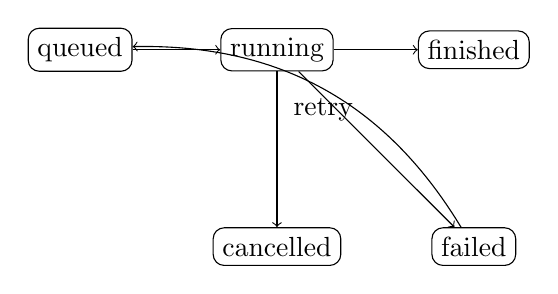
\begin{tikzpicture}[node distance=2.5cm, auto]
    \node[draw, rounded corners] (queued) {queued};
    \node[draw, rounded corners, right of=queued] (running) {running};
    \node[draw, rounded corners, right of=running] (finished) {finished};
    \node[draw, rounded corners, below of=finished] (failed) {failed};
    \node[draw, rounded corners, below of=running] (cancelled) {cancelled};
    
    \draw[->] (queued) -- (running);
    \draw[->] (running) -- (finished);
    \draw[->] (running) -- (failed);
    \draw[->] (running) -- (cancelled);
    \draw[->] (failed) edge[bend right] node[below] {retry} (queued);
\end{tikzpicture}
\caption{Job state machine transitions.}
\label{fig:job-state-machine}
\end{figure}

\subsubsection{SSE Streaming Validation}

Server-Sent Events streaming is validated for:

\begin{itemize}
    \item \textbf{Event Format}: Correct SSE format with \texttt{event:}, \texttt{data:}, and \texttt{id:} fields.
    \item \textbf{Progress Updates}: Incremental progress percentages (0--100).
    \item \textbf{Completion Events}: Final event indicates terminal status.
    \item \textbf{Connection Resilience}: Client reconnection with \texttt{Last-Event-ID} header.
\end{itemize}

\subsection{Provider Onboarding Workflow}

The provider onboarding workflow enables administrators to register and configure LLM providers.

\subsubsection{Workflow Steps}

\begin{enumerate}
    \item \textbf{Provider Registration}: \texttt{POST /v1/providers} with provider type, base URL, and credentials.
    
    \item \textbf{Model Discovery}: System queries provider for available models.
    
    \item \textbf{Instance Creation}: \texttt{POST /v1/models/instances} to configure specific model instances.
    
    \item \textbf{Default Configuration}: Set tenant/global defaults via \texttt{PATCH /v1/models/defaults}.
    
    \item \textbf{Health Monitoring}: Circuit breaker and health probes activated for provider.
    
    \item \textbf{Resilience Policies}: Configure fallback providers and cost budgets.
\end{enumerate}

\subsubsection{Validation Results}

\begin{table}[ht]
\centering
\caption{Provider onboarding validation results.}
\label{tab:provider-onboarding-results}
\small
\begin{tabular}{llc}
\hline
\textbf{Test Case} & \textbf{Description} & \textbf{Status} \\
\hline
Ollama registration & Local Ollama provider setup & \textcolor{green}{\checkmark} Pass \\
OpenAI registration & Cloud provider with API key & \textcolor{green}{\checkmark} Pass \\
Model instance creation & Create instance with custom params & \textcolor{green}{\checkmark} Pass \\
Default resolution & DMR correctly resolves user $\rightarrow$ tenant $\rightarrow$ global & \textcolor{green}{\checkmark} Pass \\
Circuit breaker init & Provider starts in CLOSED state & \textcolor{green}{\checkmark} Pass \\
Health probe & Provider health reflected in \texttt{/health/components} & \textcolor{green}{\checkmark} Pass \\
\hline
\end{tabular}
\end{table}

\subsection{Administrative Operations Workflow}

Administrative workflows are validated for tenant management, audit log access, and system configuration.

\subsubsection{Tenant Management}

\begin{itemize}
    \item \textbf{Tenant Creation}: \texttt{POST /v1/admin/tenants} creates isolated tenant context.
    \item \textbf{Configuration}: Per-tenant rate limits, model defaults, and feature flags.
    \item \textbf{Isolation}: Cross-tenant data access is blocked at the repository layer.
\end{itemize}

\subsubsection{Audit Log Access}

\begin{itemize}
    \item \textbf{Query}: Audit logs queryable by tenant, user, time range, and event type.
    \item \textbf{Immutability}: Logs are append-only; modification attempts are rejected.
    \item \textbf{Export}: Logs exportable for compliance reporting.
\end{itemize}

\subsection{End-to-End Test Execution}

E2E tests are executed using pytest with the following patterns:

\begin{lstlisting}[language=bash,caption={Running E2E tests.}]
# In-process (ASGI TestClient)
pytest -q -m "e2e"

# Against live server
docker compose up -d --build
export BASE_URL=http://localhost:8000
pytest -q -m "e2e" --live
\end{lstlisting}

\subsubsection{E2E Test Coverage}

\begin{table}[ht]
\centering
\caption{E2E test coverage by workflow.}
\label{tab:e2e-coverage}
\small
\begin{tabular}{lccc}
\hline
\textbf{Workflow} & \textbf{Test Files} & \textbf{Test Functions} & \textbf{Pass Rate} \\
\hline
Health probes & 2 & 8 & 100\% \\
Agent runs & 4 & 35 & 97\% \\
Job lifecycle & 6 & 42 & 94\% \\
Tool invocation & 35 & 280+ & 98\% \\
Provider management & 3 & 18 & 100\% \\
Admin operations & 5 & 24 & 92\% \\
\hline
\textbf{Total} & 55+ & 407+ & 96\%+ \\
\hline
\end{tabular}
\end{table}

\subsection{Workflow Diagrams}

For visual reference, the complete workflow diagrams are provided in the README documentation and reproduced in Appendix~\ref{app:api-reference}. Key flows include:

\begin{enumerate}
    \item \textbf{Agent Run Workflow}: 12-step sequence from HTTP request to final response (security middleware $\rightarrow$ intent classification $\rightarrow$ orchestration $\rightarrow$ persistence).
    
    \item \textbf{Long-Running Job Workflow}: 8-step sequence from job creation to SSE streaming completion.
    
    \item \textbf{NL-to-Cypher Pipeline}: 6-stage pipeline from natural language normalization to result summarization.
\end{enumerate}

These workflows demonstrate that the platform successfully integrates all architectural components into cohesive, production-ready user experiences.

